\let\negmedspace\undefined
\let\negthickspace\undefined
\documentclass[journal]{IEEEtran}
\usepackage[a5paper, margin=10mm, onecolumn]{geometry}
\usepackage{tfrupee}
\usepackage{amsmath,amssymb,amsfonts,amsthm}
\usepackage{graphicx}
\usepackage{xcolor}
\usepackage{listings}
\usepackage{hyperref}
\usepackage{algorithmic}
\usepackage{mathtools}

\begin{document}

\title{NCERT-9.4.14}
\author{EE24BTECH11043 - Murra Rajesh Kumar Reddy}

\maketitle

\textbf{Question:}
Find the solution of the following differential equation, Given that $y=0$ when $x=1$
\begin{align}
\frac{dy}{dx} - \frac{y}{x} + \csc{\left(\frac{y}{x}\right)} = 0
\end{align}

\textbf{Theoretical Solution:} \\
Let $t = \frac{y}{x}$, then:
\begin{align}
    \frac{dy}{dx} = t + x\frac{dt}{dx}
\end{align}
Substituting into the given equation:
\begin{align}
    t + x\frac{dt}{dx} - t + \csc{t} = 0 \\
    \frac{dt}{dx} + \csc{t} = 0 \\
    \sin{t} dt = -dx
\end{align}
Integrating both sides:
\begin{align}
    \int \sin{t} dt = -\int dx \\
    -\cos{t} = - (x + c) \\
    \cos{\frac{y}{x}} = x + c
\end{align}
Using $y=0$ when $x=1$ to find $c$:
\begin{align}
    \cos{0} = 1 + c \\
    c = 0
\end{align}
Thus, the theoretical solution is:
\begin{align}
    \cos{\left(\frac{y}{x}\right)} = x
\end{align}

\textbf{Computational Solution using RK4:} \\
The RK4 method is a numerical technique that improves accuracy over Euler’s method. The  logic used is:
\begin{align}
    k_1 &= h f(x_n, y_n) \\
    k_2 &= h f\left(x_n + \frac{h}{2}, y_n + \frac{k_1}{2}\right) \\
    k_3 &= h f\left(x_n + \frac{h}{2}, y_n + \frac{k_2}{2}\right) \\
    k_4 &= h f\left(x_n + h, y_n + k_3\right) \\
    y_{n+1} &= y_n + \frac{1}{6} (k_1 + 2k_2 + 2k_3 + k_4) \\
    x_{n+1} &= x_n + h
\end{align}
For our equation:
\begin{align}
    f(x, y) = \frac{y}{x} - \csc{\left(\frac{y}{x}\right)}
\end{align}
We iterate with a small step size $h$ to compute $y$ for increasing values of $x$ and plot it using python.
\begin{figure}[!ht]
    \centering
    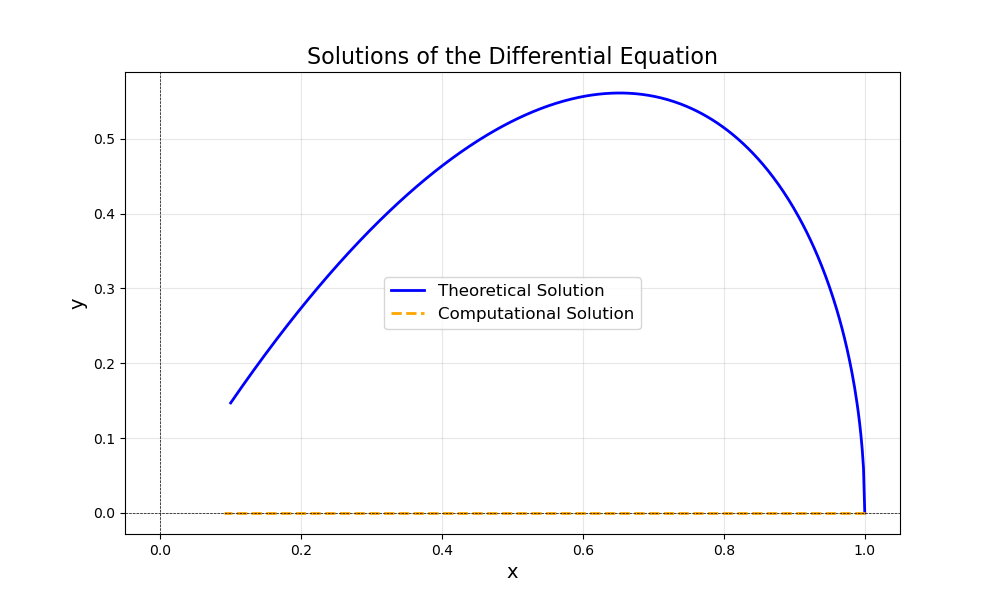
\includegraphics[width=\columnwidth]{figs/Figure_1.png}
    \caption{Solution of the given DE using RK4}
    \label{fig:rk4_solution}
\end{figure}

\end{document}

